% Image source:
% MER
% https://mars.nasa.gov/mer/

% All others:
% https://science.nasa.gov/toolkits/spacecraft-icons
This section is restricted to successful missions. At the time of writing this thesis, the \ac{NASA} remains the only organization to successfully land and operate a spacecraft on the Martian surface. Descriptions of these missions are restricted to power generation and storage characteristics.

\subsection{Landers}
\label{sec:StateOfTheArt:PastAndOngoingMissions:Landers}

Landers are shown in \refFig{fig:past-mission-landers}. The Viking Program developed orbiters and a landers. The latters, identified as \ac{VL1} and \ac{VL2}, are shown in \refFig{fig:sub:past-mission-lander-viking}. The Phoenix lander, shown in \refFig{fig:sub:past-mission-lander-phoenix}, was part of the Mars Scout Program. The ongoing \ac{InSight} mission is part of the Discovery Program and is shown in \refFig{fig:sub:past-mission-lander-insight}.

\begin{figure}[h]
\captionsetup[subfigure]{justification=centering}
\vspace{-2ex}
	\centering
    %% setup sizes
    \setlength{\subfigureWidth}{0.48\textwidth}
    \setlength{\graphicsHeight}{30mm}
    %% kill hyper-link highlighting
    \hypersetup{hidelinks=true}%
    %% the figures
	\begin{subfigure}[t]{\subfigureWidth}
        \centering
		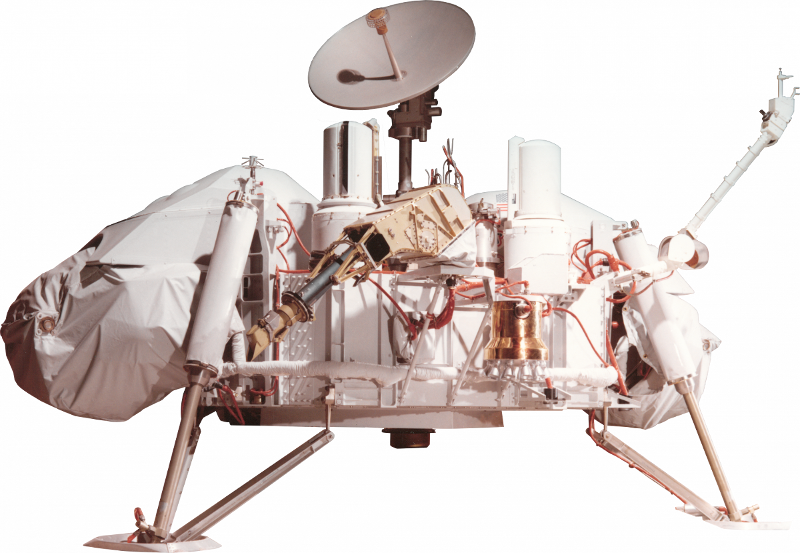
\includegraphics[height=\graphicsHeight]{sections/state-of-the-art/past-and-ongoing-missions/images/lander-viking.png}
		\subcaption{Viking}
		\label{fig:sub:past-mission-lander-viking}
	\end{subfigure}\\[0.8ex]
%% 2nd row
	\begin{subfigure}[t]{\subfigureWidth}
        \centering
		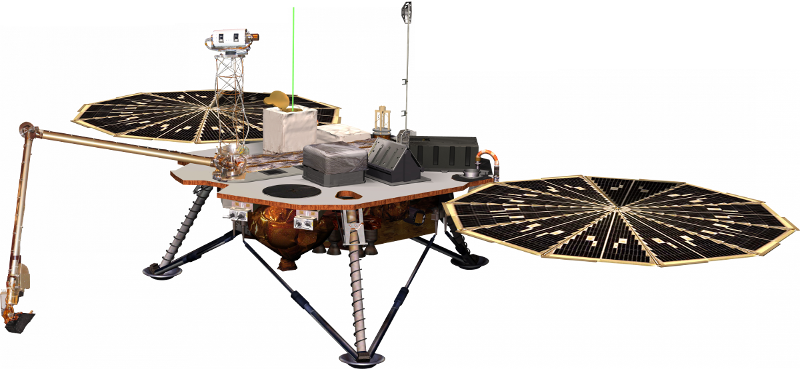
\includegraphics[height=\graphicsHeight]{sections/state-of-the-art/past-and-ongoing-missions/images/lander-phoenix.png}
        \subcaption{Phoenix}
		\label{fig:sub:past-mission-lander-phoenix}
	\end{subfigure}\hspace*{0.5cm}
    \begin{subfigure}[t]{\subfigureWidth}
        \centering
		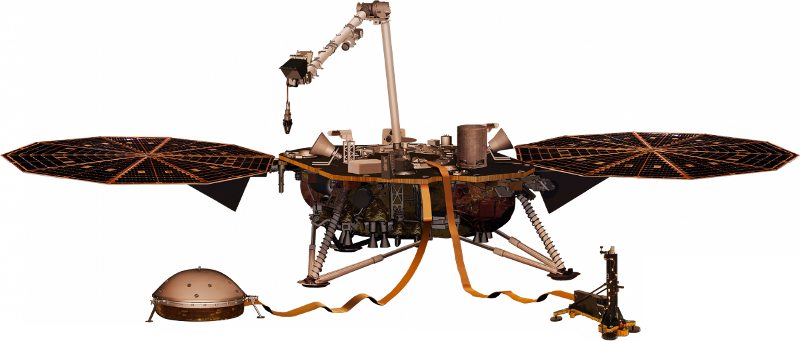
\includegraphics[height=\graphicsHeight]{sections/state-of-the-art/past-and-ongoing-missions/images/lander-insight.png}
		\subcaption{InSight}
		\label{fig:sub:past-mission-lander-insight}
	\end{subfigure}
    \caption[Past and ongoing lander missions]
            {Past and ongoing lander missions. Images: NASA.}
	\label{fig:past-mission-landers}
\vspace{-2ex}
\end{figure}

% Alternative layout of lander figures. All 3 subfigures in a single line.
\begin{comment}
\begin{figure}[h]
\captionsetup[subfigure]{justification=centering}
\vspace{-2ex}
	\centering
    %% setup sizes
    \setlength{\subfigureWidth}{0.32\textwidth}
    \setlength{\graphicsHeight}{21mm}
    %% kill hyper-link highlighting
    \hypersetup{hidelinks=true}%
    %% the figures
	\begin{subfigure}[t]{\subfigureWidth}
        \centering
		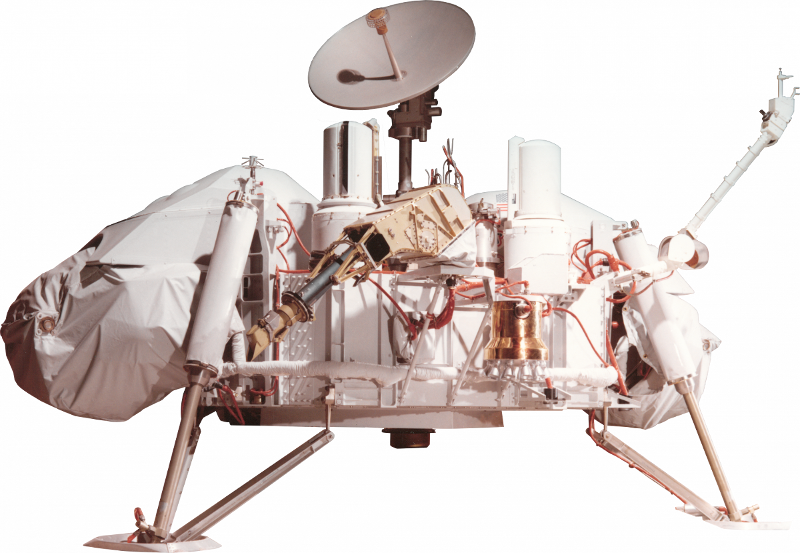
\includegraphics[height=\graphicsHeight]{sections/state-of-the-art/past-and-ongoing-missions/images/lander-viking.png}
		\subcaption{Viking Lander}
		\label{fig:sub:past-mission-lander-viking}
	\end{subfigure}\hfill
	\begin{subfigure}[t]{\subfigureWidth}
        \centering
		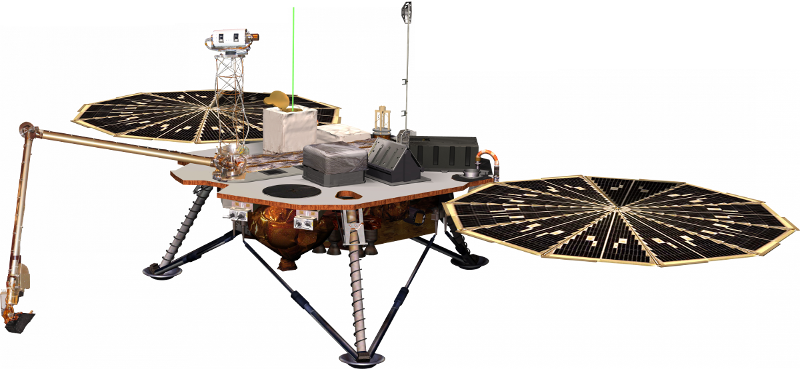
\includegraphics[height=\graphicsHeight]{sections/state-of-the-art/past-and-ongoing-missions/images/lander-phoenix.png}
		\subcaption{Phoenix Lander}
		\label{fig:sub:past-mission-lander-phoenix}
	\end{subfigure}\hfill
    \begin{subfigure}[t]{\subfigureWidth}
        \centering
		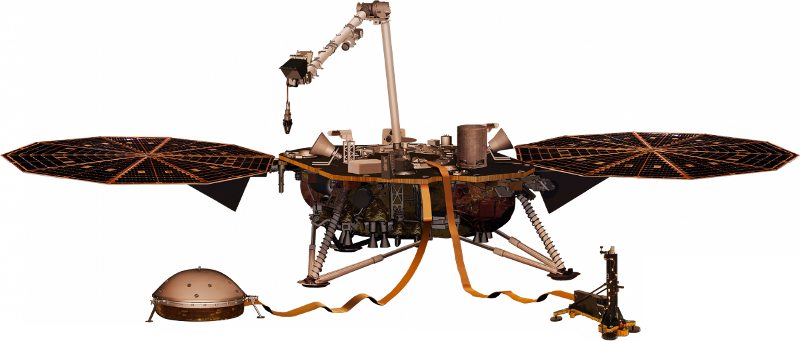
\includegraphics[height=\graphicsHeight]{sections/state-of-the-art/past-and-ongoing-missions/images/lander-insight.png}
		\subcaption{InSight Lander}
		\label{fig:sub:past-mission-lander-insight}
	\end{subfigure}
	\caption[Past and ongoing lander missions]
            {Past and ongoing lander missions.}
	\label{fig:past-mission-landers}
\vspace{-2ex}
\end{figure}
\end{comment}

\subsubsection{Viking}

A single Viking Lander was powered by two \ac{RTG} units. Converting heat from decaying plutonium-236 resulted in a continuous nominal electrical power output of \SI{70}{\watt} at \SI{4.4}{\volt}. Four \SI{30}{\volt} nominal, 42-cell \ac{NiCd} batteries were mounted in pairs and charged by the \ac{RTG} units. The battery cells were \SI{8}{\ampere\hour} at \ac{EOL}. Recharge rates depended on available \ac{RTG} energy and varied from C/40 to C/6. Descrease in charge efficieny tied to temperature increase imposed a thermal constraint in which charging did not occur if the battery temperature was greater than \SI{21}{\degree} in order to prevent excessive battery temperatures during charging. Further power subsytem design details are found in \citepower{Holmburg1980}.


\subsubsection{Phoenix}

The Phoenix Lander generated power from its two ATK ``UltraFlex'' \acp{SA} which covered a total surface area of \SI{4.2}{\meter\squared}. The \acp{SA} provided approximately \SI{22}{\watt/\kilo\gram} under Mars conditions \citepower{Badescu2009} \citeother{Linne2012}. Its round fan-fold design unfolded into two separate circular decagon panels. Two rechargeable \ac{Li-ion} \ac{NCO}-cell batteries were manufactured by Yardney and had a nameplate capacity of \SI{25}{\ampere\hour}. The battery cells were arranged in an 8s2p configuration. The battery characteristics taken from \citepower{NASAEnergyStorage2017} are as follow:

\begin{itemize}
	\item Mass: \SI{17.8}{\kilo\gram}.
	\item Operating voltage: 24\SI{32.8}{\volt}.
	\item Capacity voltage: 50‒\SI{62}{\volt}.
	\item Specific energy: \SI{105}{\watt\hour/\kilo\gram}.
    \item Operating temperature: \SI{-20}{\celsius} to +\SI{30}{\celsius}.
\end{itemize}

\subsubsection{InSight}

The InSight Lander is based on heritage from the Phoenix mission and as such shares similar characteristics. It generates power from two \acp{SA} each measuring \SI{2.2}{\meter} in diameter. The \acp{SA} are  ATK ``UltraFlex'' ZTJ triple-junction solar cells made of \ac{InGaP}/\ac{InGaAs}/\ac{Ge}. The \ac{NCA}-cells rechargeable batteries were manufactured by Yardney and based on Phoenix's NCP‒25‒1 cell design. The two 8-cell in parallel (8s2p), \SI{28}{\volt}, \SI{30}{\ampere\hour} batteries can operate down to \SI{-35}{\celsius} \citepower{EaglePitcher}. As listed in \citepower{Smart2015}, the battery performance requirements for InSight are:

\begin{itemize}
  \item The battery shall support 709 sols of surface operations over a temperature range of \SI{-30}{\celsius} to +\SI{35}{\celsius}.
  \item Each 8-cell battery shall be able to support a \SI{5}{\ampere} charge rate over the entire allowable flight temperature range of \SI{-30}{\celsius} to +\SI{35}{\celsius}.
  \item Each 8-cell battery shall provide at least \SI{25}{\ampere\hour} at \SI{-25}{\celsius} \ac{BOL} over the voltage range of \SI{24}{\volt} to \SI{32.8}{\volt} using a C/5 rate (\SI{5}{\ampere}).
\end{itemize}

\clearpage
\subsection{Rovers}
\label{sec:StateOfTheArt:PastAndOngoingMissions:Rovers}

Successful rovers are shown in \refFig{fig:past-mission-rovers}. The Sojourner rover was the first rover to operate on the Martian surface and is shown in \refFig{fig:sub:past-mission-rover-sojourner}. The \ac{MER} mission consisted of twin rovers  Spirit and Opportunity shown in \refFig{fig:sub:past-mission-rovers-mer}. The ongoing \ac{MSL} Curiosity mission is part of the \ac{MEP} and shown in \refFig{fig:sub:past-mission-rovers-msl}.

\begin{figure}[h]
\captionsetup[subfigure]{justification=centering}
\vspace{-2ex}
	\centering
    %% setup sizes
    \setlength{\subfigureWidth}{0.45\textwidth}
    \setlength{\graphicsHeight}{35mm}
    %% kill hyper-link highlighting
    \hypersetup{hidelinks=true}%
    %% the figures
	\begin{subfigure}[t]{\subfigureWidth}
        \centering
        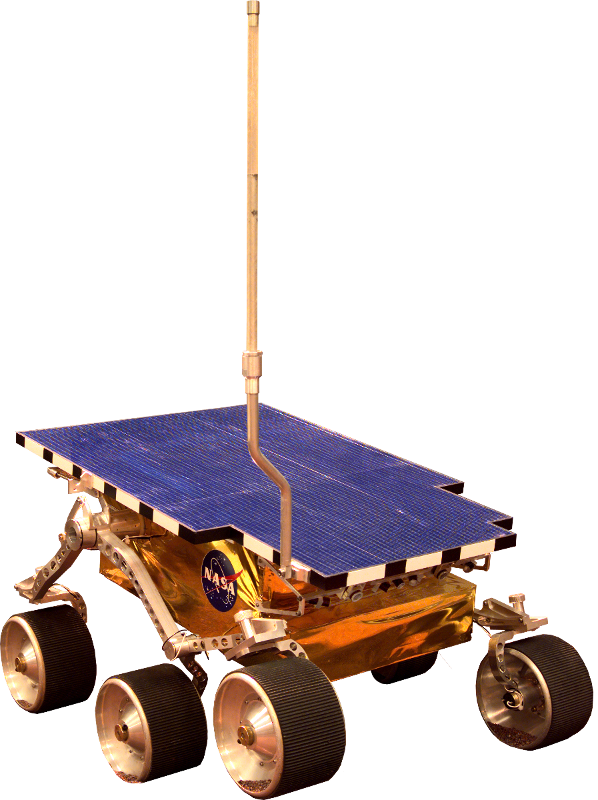
\includegraphics[height=\graphicsHeight]{sections/state-of-the-art/past-and-ongoing-missions/images/rover-sojourner.png}
        \subcaption{Sojourner}
        \label{fig:sub:past-mission-rover-sojourner}
	\end{subfigure}\\[0.8ex]
%% 2nd row
	\begin{subfigure}[t]{\subfigureWidth}
        \centering
		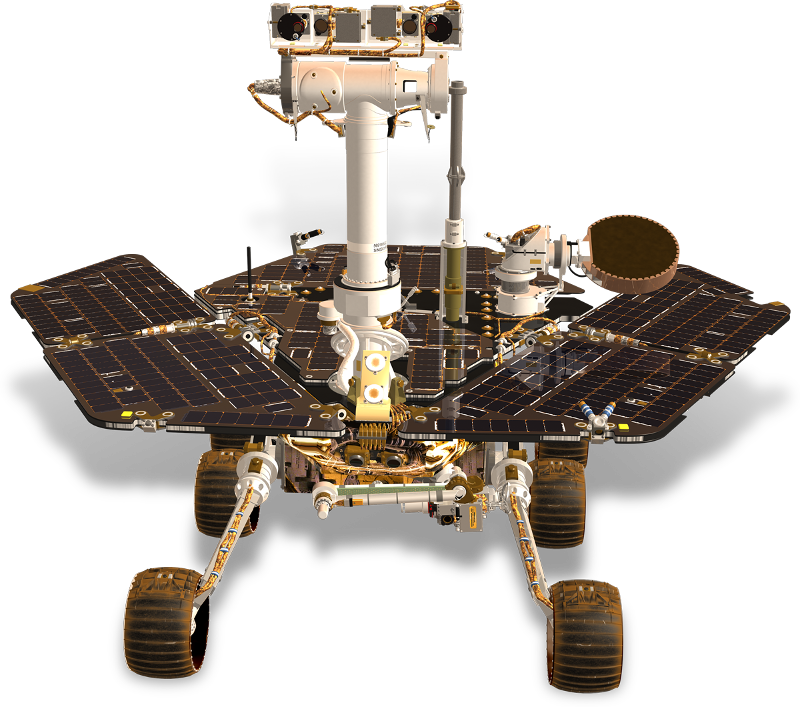
\includegraphics[height=\graphicsHeight]{sections/state-of-the-art/past-and-ongoing-missions/images/rover-mer.png}
		\subcaption{MER Opportunity and Spirit}
		\label{fig:sub:past-mission-rovers-mer}
	\end{subfigure}\hspace*{0.5cm}
    \begin{subfigure}[t]{\subfigureWidth}
        \centering
		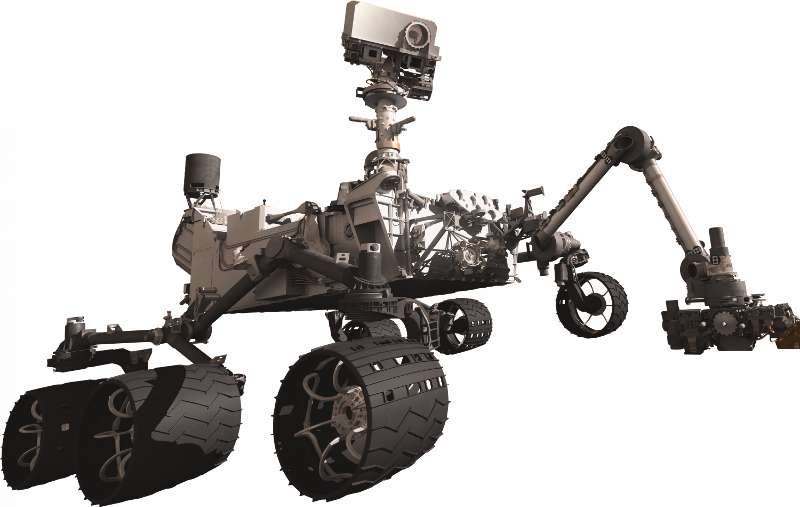
\includegraphics[height=\graphicsHeight]{sections/state-of-the-art/past-and-ongoing-missions/images/rover-msl.png}
		\subcaption{MSL Curiosity}
		\label{fig:sub:past-mission-rovers-msl}
	\end{subfigure}
    \caption[Past and ongoing rover missions]
            {Past and ongoing rover missions. Images: NASA.}
	\label{fig:past-mission-rovers}
\vspace{-2ex}
\end{figure}

\begin{comment}

\vspace{0.5cm}

\begin{figure}[h]
\captionsetup[subfigure]{justification=centering}
\vspace{-2ex}
	\centering
    %% setup sizes
    \setlength{\subfigureWidth}{0.32\textwidth}
    \setlength{\graphicsHeight}{30mm}
    %% kill hyper-link highlighting
    \hypersetup{hidelinks=true}%
    %% the figures
	\begin{subfigure}[t]{\subfigureWidth}
        \centering
		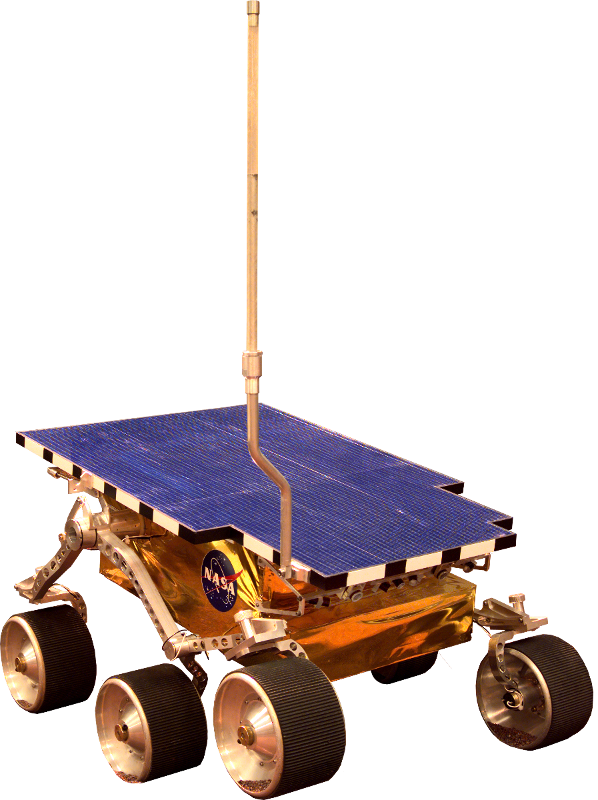
\includegraphics[height=\graphicsHeight]{sections/state-of-the-art/past-and-ongoing-missions/images/rover-sojourner.png}
		\subcaption{Sojourner}
		\label{fig:sub:past-mission-rover-sojourner}
	\end{subfigure}\hfill
	\begin{subfigure}[t]{\subfigureWidth}
        \centering
		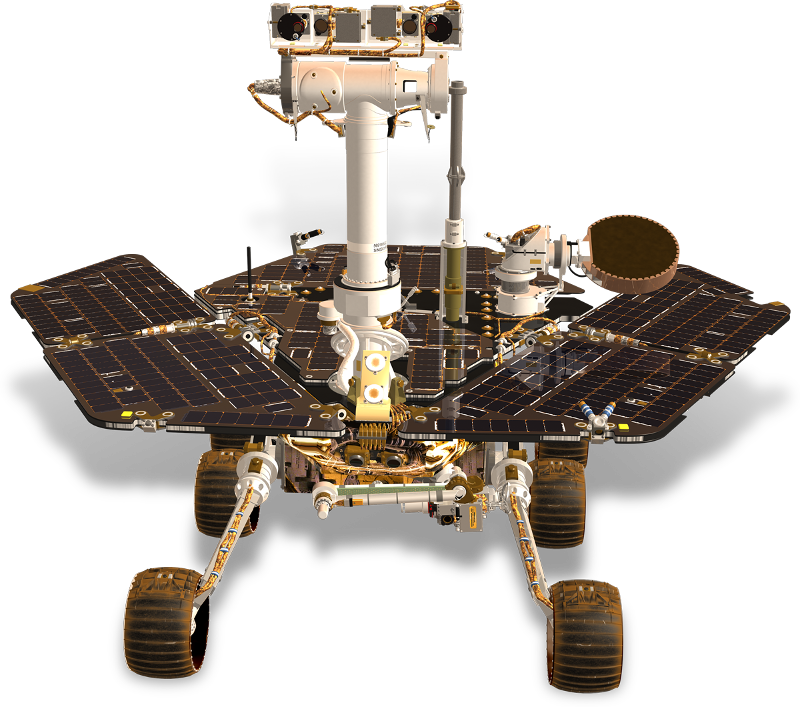
\includegraphics[height=\graphicsHeight]{sections/state-of-the-art/past-and-ongoing-missions/images/rover-mer.png}
		\subcaption{MER Opportunity and Spirit}
		\label{fig:sub:past-mission-rovers-mer}
	\end{subfigure}\hfill
    \begin{subfigure}[t]{\subfigureWidth}
        \centering
		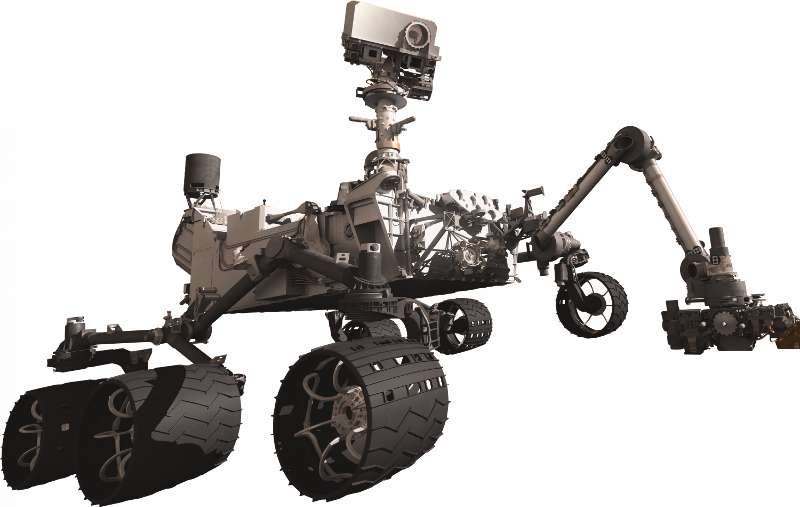
\includegraphics[height=\graphicsHeight]{sections/state-of-the-art/past-and-ongoing-missions/images/rover-msl.png}
		\subcaption{MSL Curiosity}
		\label{fig:sub:past-mission-rovers-msl}
	\end{subfigure}
	\caption[Past and ongoing rover missions]
            {Past and ongoing rover missions.}
	\label{fig:past-mission-rovers}
\vspace{-2ex}
\end{figure}
\end{comment}

\subsubsection{Sojourner}
The Sojourner microrover was powered by a 0.22\si{\meter\squared}, $\SI{2}{\centi\meter}\times\SI{4}{\centi\meter}$, 5.5 mil thick \ac{GaAs}/\ac{Ge} solar panel. Its operating temperature was from \SI{-140}{\celsius} to +\SI{110}{\celsius}. Each of its three batteries were configured as 3 \ac{Li-SOCL2} D-size cells arranged in series and provided up to \SI{150}{\watt\hour}. The battery cell capacity was \SI{12}{\ampere\hour} at +\SI{25}{\celsius} and \SI{8}{\ampere\hour} at \SI{-20}{\celsius}. Operating voltage was 8‒11 \si{\volt} and mass was 1.24 \si{\kilo\gram}. The rover's power system allowed it to draw of up \SI{30}{\watt} of peak power with a peak solar panel power output of \SI{16}{\watt}. The rover's nominal propulsion power requirement is \SI{10}{\watt}. Further details on Sojourner's power subsystem are found in \citepower{SojournerDescription} and \citepower{SojournerPowerSubsystem}.

\subsubsection{Opportunity and Spirit}
The twin rovers generated power from their \ac{TJ} \ac{GaInP}/\ac{GaAs}/\ac{Ge} \acp{SA} with a solar cell coverage area of \SI{1.3}{\square\meter}. The \acp{SA} could generate almost \SI{900}{\watt\hour} of energy at \ac{BOL} on a clear day in absence of dust deposition \citepower{Badescu2009}. The rovers's propulsion power draw was approximately \SI{100}{\watt}. Two rechargeable \ac{Li-ion} NCP-8-1 \ac{NCO}-cell batteries were manufactured by Yardney and provided support to the \ac{SA} as well as enabled nighttime experiments \citepower{Badescu2009}. Each battery was configured in 8-cell \SI{10}{\ampere\hour} strings connected in parallel (8s2p). The nameplate capacity was \SI{8}{\ampere\hour} and the \ac{DOD} was designed to typically be 40‒50 \si{\percent} per Sol \citepower{Gulbinska2014}. The battery characteristics taken from \citepower{NASAEnergyStorage2017} are as follow:

\begin{itemize}
	\item Mass: \SI{7.12}{\kilo\gram}.
	\item Operating voltage: 24‒\SI{32.8}{\volt}.
	\item Capacity voltage: 16‒\SI{20}{\volt}.
	\item Specific energy:\SI{90}{\watt\hour/\kilo\gram}.
    \item Operating temperature: \SI{-20}{\celsius} to +\SI{30}{\celsius}.
\end{itemize}

The rovers were heated by eight \acp{RHU}, each of which continuously generated \SI{1}{\watt} of thermal energy. The following are notable battery operational requirements taken from \citepower{Gulbinska2014}:

\begin{itemize}
  \item Maintaining the operating voltage of 24‒36 \si{\volt}.
  \item Providing sufficient energy for surface operations ($\geq$ \SI{283}{\watt\hour} per Sol at \SI{0}{\celsius}).
  \item Delivering sufficiently long cycle life ($\geq$ 270 cycles at \SI{50}{\percent} \ac{DOD} and/or 90 Sols operation).
  \item The battery should successfully charge and discharge between -20 and +\SI{30}{\celsius} throughout the length of the entire mission.
\end{itemize}

\subsubsection{Curiosity}
The Curiosity rover uses the \ac{MMRTG} power system. It is designed to initially provide around \SI{2000}{\watt} of thermal power and \SI{110}{\watt} of electrical power in a deep space environment \citepower{MMRTG}. The electrical output is used to charge its two Yardney \ac{Li-ion} NCP-42-1 \ac{NCO}-cell batteries, which have a nameplate capacity rating of \SI{42}{\ampere\hour}. Curiosity's battery cells are arranged in an 8s2p configuration. The battery characteristics taken from \citepower{NASAEnergyStorage2017} are as follow:

\begin{itemize}
   \item Mass: \SI{26.5}{\kilo\gram}
   \item Operating voltage: 24‒\SI{32.8}{\volt}.
   \item Capacity voltage: 86‒\SI{92}{\volt}.
   \item Specific energy:\SI{104}{\watt\hour/\kilo\gram}.
   \item Operating temperature: \SI{-20}{\celsius} to +\SI{30}{\celsius}.
\end{itemize}

The following are notable battery performance requirements taken from \citepower{Smart2009}:

\begin{itemize}
  \item Operation for more than 40 months after launch and a calendar life of $>$ 4 years.
  \item Provide 670 cycles of up to \SI{310}{\watt\hour} at 0‒\SI{30}{\celsius}, with a \SI{22}{\ampere} max capability to \SI{25}{\volt}.
  \item Provide 670 cycles of up to \SI{295}{\watt\hour} at -20 to +\SI{30}{\celsius}, with a \SI{10}{\ampere} max to \SI{25}{\volt}.
  \item Provide 670 cycles of up to \SI{555}{\watt\hour} at 0 to +\SI{30}{\celsius}, with a \SI{22}{\ampere}  max to \SI{25}{\volt} (only once per Martian Sol).
  \item Possess capability of meeting the performance requirements with an average battery temperature of +\SI{15}{\celsius} and an absolute maximum of +\SI{30}{\celsius} on the surface of Mars.
\end{itemize}
